\documentclass{article}
\usepackage{amsmath, amssymb}
\usepackage{mathtools} % for smashoperator
\usepackage{hyperref}
\hypersetup{
    colorlinks=true,
    linkcolor=cyan,
    citecolor=magenta,
    filecolor=magenta,
    urlcolor=cyan,
    runcolor=cyan,
}

% Bibliography
\usepackage[
backend=biber,
style=phys,
biblabel=brackets
]{biblatex}

\addbibresource{allrefs.bib}
\addbibresource{/home/pawel/Documents/Zotero/pawels_library.bib}
% End bibliography

\title{
    Vibronic effects in the absorption spectra of strontium phenoxide, SrOPh,
    and its deuterated version, SrOPh-d$_5$
}

\author{..., Paweł Wójcik, ...}

\begin{document}
\maketitle

\section{Introduction}
\label{sec:intro}

This document presents simulation of the absorption spectra of strontium
phenoxide and its deuterated version: SrOPh, SrOPh-d$_5$. Both molecules belong of
the family of second-group metal organic-mono-oxides, which are characterized
by an alkali-atom-like spectrum induced by the presence of a single unpaired
electron localized at the metal atom. The molecular ground state $\tilde{X}^2 A
_1$ corresponds to the hydrogen-atom-like (5s$^1$) $^2$S state of Rb. The pair
of molecular states, $\tilde{A} ^2 B_{2}$ and $\tilde{B} ^2 B _{1}$,
corresponds to two of the triply-degenerate (5p$^1$) $^2$P states, where the
degeneracy is lifted by the lowered symmetry of the molecule. The $\tilde{C} ^2
A _1$ state corresponds to the third component of $^2 P$ state, which would
extend towards the phenoxide ligand, and as such it is more mixed and shows a
larger energy gap.

All four states are characterized by very similar equilibrium structures and
very similar potential energy surfaces, which results in almost no changes to
the vibrational state during radiative decay of the excited states. 

The lowest frequency modes are vibrations of the M-O-C group. In case of SrOPh,
the three lowest frequency modes, in order are: the in-plane M-O-C bend, $\nu
_{33} (b _2)$, the out-of-plane M-O-C bend, $\nu _{22} (b _1)$, and the M-O
stretch, $\nu _{12} (a _1)$. There is at least one more set of higher frequency
modes that has a significant component along each of these three motions. The
deuterated molecule shares similar traits.

Out of these three types of motion, the best studied one is the M-O stretch.
The reason behind it lies in the extensively studied fluorescence spectrum of
the vibrationless $\tilde{A}$ or $\tilde{B}$ states. Such spectra shows
progressions in the M-O stretching modes which are attributed to the changes in
the M-O bond length between the electronic states; the most prominent, although
very small, geometrical relaxation.

This work focuses on the states that lie above the vibrational ground state of
the $\tilde{A}$ state, all the way up in the energy range past the $\tilde{B}$
state, a region spanning about $700$~cm$^{-1}$. In this region, the M-O
stretching modes remain highly relevant and prominent, however, it is also the
range where the M-O-C bending modes exhibit its significance as the carriers of
the vibronic couplings. 

The presence of the vibronic couplings stresses that the description of the
vibronic states as products of an electronic state and a vibrational state is
no longer valid. The vibronic states, which are the eigenstates of the
molecular Hamiltonian, show mixing of various electronic states used in the
zeroth-order model described above. This work simulates the vibronic states
using the K\"oppel-Domcke-Cederbaum (KDC) Hamiltonian and discusses the
consequences of the mixing on the fluorescence spectra and prospects of optical
cycling.

\section{Methods}
\label{sec:methods}

The methods used in this work were recently successful in simulations of
vibronic effects in other molecules, in particular for YbOH, CaOH, SrOH, RaOH,
SrOCH$_3$, SrNH$_2$, NO$_3$, benzene cation, O$_3$, and
pyrazine.\autocite{Doyle:YbOH:20, zhangAccuratePredictionMeasurement2021,
Doyle:SrOH:22, zhangIntensityborrowingMechanismsPertinent2023,
frenettVibrationalBranchingFractions2024, Stanton:NO3:07, Koppel:02,
Wojcik:ozone:2024} The specific shape of the quantum chemistry models and the
vibronic Hamiltonian used in this work is described below.

The electronic structure calculations use the coupled-cluster (CC) based
methods.~\autocite{Bartlett:CC_review:07} In particular we use the electron
attachment flavor of the equation-of-motion extension of CC truncated to single
and double substitutions (EOM-EA-CCSD).~\autocite{Krylov:EOMRev:07,
Bartlett:Book:09, Christiansen:EOMRev:11, Bartlet:EOMRev:12, Krylov:OSRev}

We compute the vertical excitation energies $E ^{(\alpha)}$ using composite
schemes involving basis set extrapolation and use of EOM-CC truncated to
include full single, double, and perturbative triple excitations
(EOM-CCSD$^*$), where the highest level of theory was especially needed for the
$\tilde{C}$ state.~\autocite{StantonGauss:SD3:96} All CC calculations were
carried out in \textsc{CFOUR} and \textsc{Q-Chem}.~\autocite{cfour, cfour:2020,
qchem_feature, qchem5_full} We did not invoke the frozen-core approximation ---
all electrons were included in the correlated calculations.

The vibronic simulations use the KDC Hamiltonian.~\autocite{Cederbaum:LVC:84,
KDC:81, Koppel:CIbookCh7:04} The KDC Hamiltonian is designed for use in a basis
of diabatic states which for which we use the definition of Ichino, Gauss, and
Stanton.~\autocite{Stanton:EOMIPdeg:09} 

The KDC Hamiltonian (expanded in the dimensionless normal coordinates of the
ground state)
\begin{equation}
    H _{KDC} = 
    H _0 \mathbf{1}
    +
    \begin{bmatrix}
    V ^{(\tilde{A})} & V ^{(\tilde{A}\tilde{B})} & V ^{(\tilde{A}\tilde{C})} \\
    V ^{(\tilde{B}\tilde{A})} & V ^{(\tilde{B})} & V ^{(\tilde{B}\tilde{C})} \\
    V ^{(\tilde{C}\tilde{A})} & V ^{(\tilde{C}\tilde{B})} & V ^{(\tilde{C})} \\
    \end{bmatrix},
    \label{eq:kdc}
\end{equation}
consists of the diagonal harmonic terms
\begin{equation}
    H _0 = -\frac{1}{2} \sum _{i = 1} ^ {N _{nm}} 
    \omega _i 
    \left(
    \partial ^2 _{Q _i}
    + 
    Q _i ^ 2
    \right),
    \label{eq:kdc_H0}
\end{equation}
the diagonal diabatic potential terms
\begin{equation}
    V ^{(\alpha)} 
    = 
    E ^{(\alpha)}
    +
    \sum _{i = 1} ^ {N _{nm}} 
    \kappa _i ^{(\alpha)}
    Q _i
    \label{eq:kdc_Vdiag}
\end{equation}
and the off-diagonal, diabatic coupling terms
\begin{equation}
    V ^{(\alpha\beta)} 
    = 
    \smashoperator{\sum _{i \in \{\text{coupling modes}\}}}
    \lambda _i ^{(\alpha \beta)}
    Q _i.
    \label{eq:kdc_Voff}
\end{equation}
$N _{nm}$ is the number of normal modes included in the model. $\mathbf{1}$ is
a $3 \times 3$ identity matrix. $\omega _i$ is the ground state harmonic
frequency of the normal mode $i$. $Q_i$ is a dimensionless normal coordinate.
$E ^{(\alpha)}$ is the vertical excitation energy of the electronic state
$\alpha$. $\kappa ^{(\alpha)} _i$ is energy gradient of state $\alpha$ along
the dimensionless normal mode $i$. $\lambda ^{(\alpha \beta)} _i$ is the linear
diabatic coupling constant between states $\alpha$ and $\beta$ along normal
mode $i$.

Using definition of (quasi)-diabatic states given by Ichino, Gauss, and
Stanton, the linear diabatic coupling constants, $\lambda ^{(\alpha \beta)}
_i$, were computed \emph{ab initio}.~\autocite{Stanton:EOMIPdeg:09} Along fully
symmetric modes, where the diabatic potential coincides with the adiabatic
potential, the linear expansion coefficients $\kappa ^{(\alpha)} _i$ were
calculated \emph{ab initio} using the EOM-CCSD analytic gradients, while along
the non-fully-symmetric modes these coefficients vanish as all states were
found to have planar $C_{2v}$ symmetry.~\autocite{StantonGauss:EOMgrad:94}

We simulate the vibronic spectrum with the \textsc{xsim}
program.~\autocite{Sharma:xsim_socjt:2024} The vibronic simulations used 15
basis set functions per vibrational mode and 2000 Lanczos iterations.
 
The ground-state geometry was optimized using EOM-EA-CCSD. The SrOPh geometry
was optimized using EOM-EA-CCSD/cc-PVDZ[H,C,O]/cc-pwCVDZ-DK2[Sr]. The
calculations of the harmonic frequencies, potential expansion coefficients
$\kappa$ and linear diabatic couplings $\lambda$, were carried out at the same
level of theory.

The calculation of the vertical excitation energies $E ^{(\alpha)}$ were
carried out using a composite scheme: the EOM-EA-CCSD energies were calculated
using a series of basis sets and extrapolated to the complete basis set (CBS)
limit. The higher correlation effect was added by calculating the difference
between the EOM-EA-CCSD$^*$ and EOM-EA-CCSD energies, and the difference was
applied to the energies as a triples correction. The spin-orbit couplings (SOC)
were calculated between the $\tilde{X}$, $\tilde{A}$, $\tilde{B}$, and
$\tilde{C}$ states, the SOC Hamiltonian was constructed and diagonalized (see
SI of Ref.~\cite{Khvorost:dualOCC:2024} for details) to yield the final
values of the vertical excitation energies.

In the multistate and multimode KDC Hamiltonian three excited electronic states are coupled: $\tilde{A}$, $\tilde{B}$, and $\tilde{C}$. A varying number of normal modes is included throughout the simulations in order to observe the impact of various modes on the vibronic spectrum. All 33 normal modes cannot be included in the simulation as this leads to numerically intractable problem. The parameters of the KDC Hamiltonian are expanded around the ground state's equilibrium geometry.

The molecular orientation and normal mode labels follow the Mulliken's
convention.~\autocite{Mulliken:55:symnot} The molecule is oriented in the
$yz$-plane with the symmetry axis along the $z$ axis. The normal modes are
ordered first by their symmetry: $a_1$, $a_2$, $b_1$, $b_2$. Within each
symmetry block the modes are ordered by their harmonic frequencies in a
decreasing order. Out of the 33 normal modes of the molecule 12 transforms with
$a _1$ irrep, 3 with $a_2$, 7 with $b _1$, and 11 with $b _2$.

\section{Results}

This section opens with description of the parameters that enter the KDC
Hamiltonian and moves to the description of the simulated spectra focusing on
the appearance of the vibronic features.

\subsection{Parameters of the KDC Hamiltonian}
\label{sec:results:parameters}

\begin{table}
    \center
    \begin{tabular}{|c|c|c|c|c|}
        \hline
    $E ^{(\alpha)}$ & aug-cc-pwCVDZ & aug-cc-pwCVTZ & aug-cc-pwCVQZ & CBS \\
        \hline
    $\tilde{A}$ &   14288 &   14501 &   14512 &   14520 \\
    $\tilde{B}$ &    +195 &    +169 &    +167 &    +165 \\
    $\tilde{C}$ &   +1966 &   +1668 &   +1615 &   +1577 \\
        \hline
    \end{tabular}
    \caption{
        Vertical excitation energies for the SrOPh in cm$^{-1}$. The first row
        presents the energy of the $\tilde{A}$ state while the rows for the
        $\tilde{B}$ and $\tilde{C}$ states show the energy gap above the
        $\tilde{A}$ state. Calculated using EOM-EA-CCSD and correlating all
        electrons, with pseudopotential for the core Sr electrons ECP28MDF.
    }
    \label{tab:sroph_vertical_cbs}
\end{table}

\begin{table}
    \center
    \begin{tabular}{|c|c|c|c|c|}
        \hline
    $E ^{(\alpha)}$ & EOM-CCSD/CBS & $\Delta$EOM-CCSD$^*$ & SOC & final \\
        \hline             
    $\tilde{A}$ &  14520       &  +40 & -73 & 14487 \\
    $\tilde{B}$ &  14685       &  +24 & +53 & 14762 \\
    $\tilde{C}$ &  16097       & -209 & +10 & 15898 \\
        \hline
    \end{tabular}
    \caption{
        Vertical excitation energies for the SrOPh in cm$^{-1}$. Corrections
        due to the triples correlation ($\Delta$EOM-EA-CCSD$^*$) and spin-orbit
        couplings.
    }
    \label{tab:sroph_vertical_dT_SOC}
\end{table}

The parameters of the KDC Hamiltonian, Eq.~\eqref{eq:kdc}, are expanded around
the optimized geometry of the $\tilde{X}$ state. This section first presents
the vertical excitation energies, then the harmonic frequencies, and the
couplings.

The vertical excitation energies were calculated using a composite scheme
discussed in the Sec.~\ref{sec:methods}. Table~\ref{tab:sroph_vertical_cbs}
lists the vertical excitation energies and their CBS limit. The main
observation is that the quadruple-$\zeta$-quality basis is within
$10$~cm$^{-1}$ from the CBS limit for the $\tilde{A}$ and $\tilde{B}$ state and
about five times as far for the $\tilde{C}$ state.
Table~\ref{tab:sroph_vertical_dT_SOC} lists the corrections due to higher
correlation effects and the SOCs. The triples correction are of the order of
tens of wavenumbers for the $\tilde{A}$ and $\tilde{B}$ states, and again a
much larger for the $\tilde{C}$ state. The SOCs repel the $\tilde{A}$ and
$\tilde{B}$ state by more than $100$~cm$^{-1}$. The SOCs do not shift the
energy of the $\tilde{C}$ state by much, however, the $\tilde{C}$ state might
interact more strongly with the higher states that are not included in this
model. The right-most column of Table~\ref{tab:sroph_vertical_dT_SOC} shows the
final values of this composite scheme, these values are also plotted on
figure~\ref{fig:SrCouplings}.

All remaining parameters of the model are expanded in the basis of normal modes
of the ground state. The harmonic frequency of the fully symmetric stretch,
$\nu _{12} (a_1)$ is $239$~cm$^{-1}$. The harmonic frequencies of the
non-fully-symmetric modes are: $65$~cm$^{-1}$ for the in-plane Sr-O-C bend,
$\nu _{33}(b_2)$, and $84$~cm$^{-1}$ for the out-of-plane Sr-O-C bend, $\nu
_{22} (b _1)$. The next mode, in the order of increasing frequency, $\nu _{21}
(b _1)$, has the frequency $273$~cm$^{-1}$ and is also largely an out-of-plane
Sr-O-C bend. These four modes, their combinations, and their couplings produce
most of the vibronic features in the region between and close to the
$\tilde{A}$, and $\tilde{B}$ states, which in this model are separated by the
vertical gap of $275$~cm$^{-1}$.

\begin{figure}
    \begin{center}
        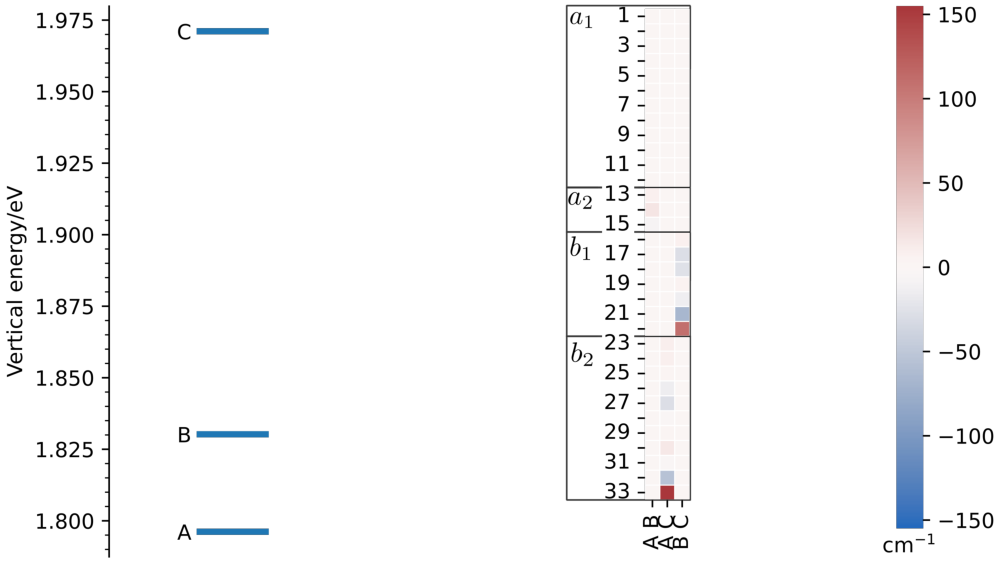
\includegraphics[width=12 cm]{./figures/SrCoupplings.pdf}
    \end{center}
    \caption{
        Left: vertical excitation energies, i.e., $E ^{(\alpha)}$s from
        Eq.~\eqref{eq:kdc_Vdiag}. Right: Linear diabatic couplings, i.e.,
        $\lambda$s from Eq.~\eqref{eq:kdc_Voff}, for SrOPh. 
    }
    \label{fig:SrCouplings}
\end{figure}

Figure~\ref{fig:SrCouplings} presents the structure of the linear diabatic
couplings for SrOPh. The couplings between $\tilde{A}$ and $\tilde{C}$ states
(middle column) are the strongest along the in-plane Sr-O-C bending modes,
these are the modes displacing the Sr and O atoms into the electronic density
of the unpaired electron in the $\tilde{A}$ state. Similarly, the $\tilde{B}$
and $\tilde{C}$ states couple along the out-of-plane Sr-O-C modes. The linear
vibronic coupling constants between $\tilde{A}$ and $\tilde{B}$ states are
vanishingly small. The coupling between these two, closely-lying states appear
in this model in second-order, e.g., through a vibronically active combination
modes.

\subsection{Vibronic simulation results}
\label{sec:results:simulations}

\begin{figure}
    \begin{center}
        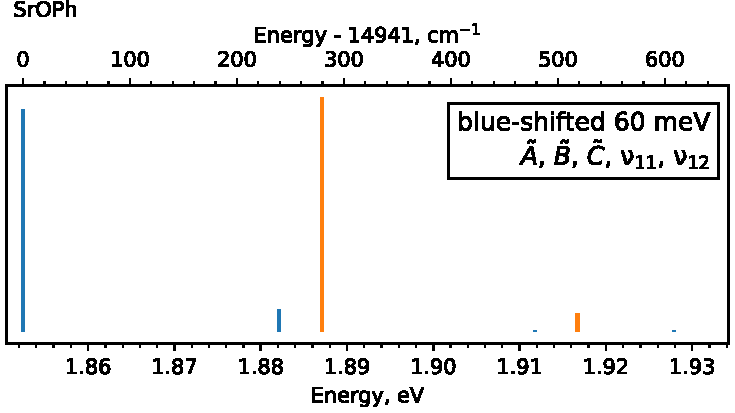
\includegraphics[width=12 cm]{figures/SrOPh_0t650_no_couplings.pdf}
        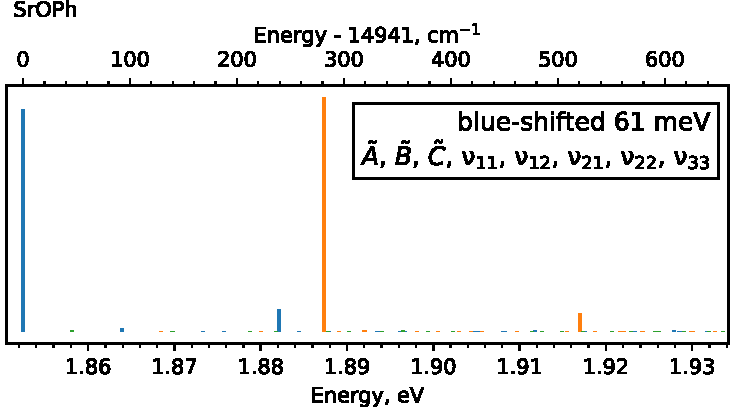
\includegraphics[width=12 cm]{figures/SrOPh_0t650.pdf}
    \end{center}
    \caption{
        Simulated absorption spectrum of SrOPh. The top spectrum displays the
        no-couplings case (Franck-Condon simulation). Colors mark symmetry of
        the vibronic peaks: blue B$_2$, orange B$_1$, green A$_1$. The inset
        box marks the states and modes active in the simulation.
    }
    \label{fig:SrOPh_0t650}
\end{figure}

\begin{figure}
    \begin{center}
        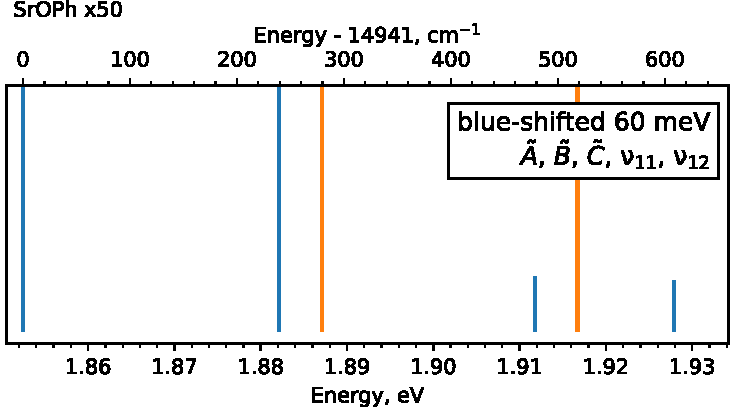
\includegraphics[width=12 cm]{figures/SrOPh_0t650_no_couplings_zoom.pdf}
        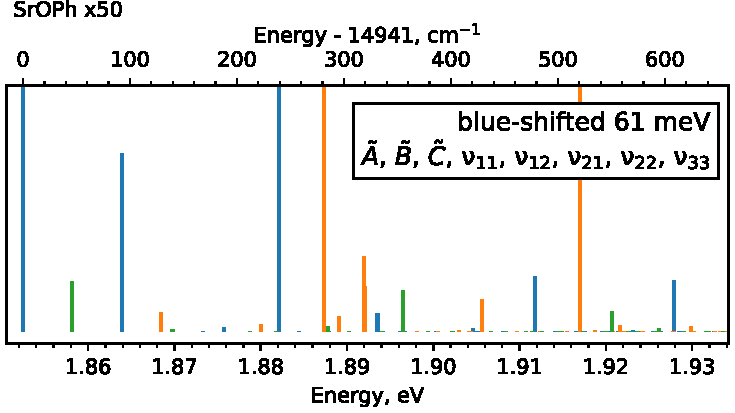
\includegraphics[width=12 cm]{figures/SrOPh_0t650_zoom.pdf}
    \end{center}
    \caption{
        A blow-up version of figure~\ref{fig:SrOPh_0t650}.
    }
    \label{fig:SrOPh_0t650_zoom}
\end{figure}

The role of the vibronic effects in the simulated spectrum is best presented
when the vibronic spectrum is compared against the simulation which does not
include the vibronic couplings, see figure~\ref{fig:SrOPh_0t650}.

The uncoupled spectrum is typical for a laser-coolable molecule. The most
prominent peak in the spectrum corresponds to the electronic transition which
does not change the vibrational state. The key transitions which change the
vibrational state excite the $\nu _{12}$ mode, i.e., the mode with a
significant Sr-O stretching component. The progression in $\nu _{12}$ is
present both in the $\tilde{A}$ and $\tilde{B}$ states, but the peaks'
intensities make less than $10$~\% of the 0-0 peak's intensity. Both
simulations also show the small $\nu _{11} (a _1)$ peak close to the
$600$~cm$^{-1}$ mark, that corresponds to the second, lowest-frequency mode
with the Sr-O stretching component. This is a complete description of the major
features of the spectrum visible up to about the first $600$~cm$^{-1}$. The
simulation which neglects the vibronic couplings reproduces these features very
well. A closer inspection of the spectrum, however, reveals an important role
of the vibronic couplings.

\begin{figure}
    \begin{center}
        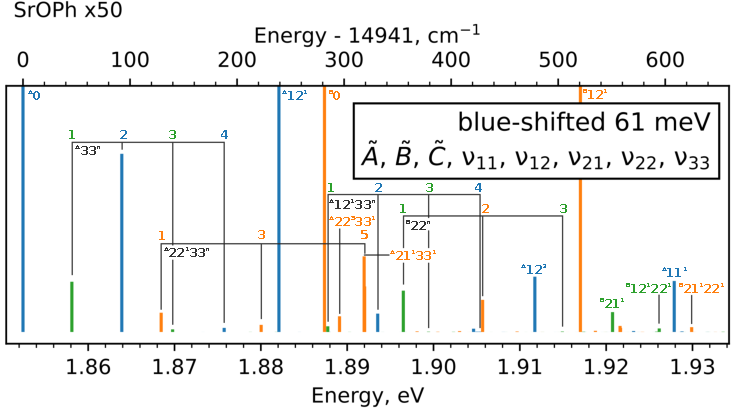
\includegraphics
        [width=12 cm]
        {figures/SrOPh_0t650_zoom_annot_Mulliken.pdf}
    \end{center}
    \caption{
        Simulated vibronic spectrum with annotations marking peak's
        assignments. The assignments corresponds to the leading term in the
        states which are mixed due to the vibronic couplings. Colors mark
        symmetry of the vibronic peaks: blue B$_2$, orange B$_1$, green A$_1$.
    }
    \label{fig:SrOPh_0t650_assigned}
\end{figure}

The role of figure~\ref{fig:SrOPh_0t650_zoom} is to bring focus to the finer
features of the vibronic spectrum; features which are missing in the uncoupled
simulation. This spectrum reveals a massive enhancement in the number of
vibronic states that are weakly allowed as a consequence of the vibronic
effects. The KDC-Hamiltonian-based simulations reveal that there are two
mechanisms leading to the appearance of these features: the direct and
second-order vibronic couplings.

\subsubsection{The direct coupling of the $\tilde{A}$ and $\tilde{B}$ states to
the $\tilde{C}$ state} 
\label{sec:results:simulations:linear}

The first vibronic effect is an appearance of progressions directly resulting
from the linear vibronic coupling model. Figure~\ref{fig:SrOPh_0t650_assigned}
helps in this discussion by presenting an assignment of the vibronic features
of the fully \emph{ab initio} simulated spectrum. The assignments appear as a
Franck-Condon-type decoupled state labels, but these are only used to mark the
leading terms in the otherwise mixed state. The linear vibronic couplings model
used in this work is based on diabatic couplings between electronic states.
These couplings appear between pairs of electronic states as expansion
coefficients along non-fully-symmetric modes as presented on
figure~\ref{fig:SrCouplings}. Such modes are inactive in the uncoupled, i.e.,
Franck-Condon simulation. The couplings allow for mixing of electronic states
along the coupling modes. 

The lowest-energy progression of this type appears for the $\nu _{33}$ mode
(in-plane Sr-O-C bending) and is labeled $^{\tilde{A}}33^n$ on
figure~\ref{fig:SrOPh_0t650_assigned}. The symmetry of vibronic peaks in this
progression changes between the symmetry of the ``host'', $\tilde{A}$
electronic state (for even number of quanta) and of the ``coupled'',
$\tilde{C}$ electronic state (for odd number of quanta). This progression
differs from a typical Franck-Condon progression in the peaks' intensity
distribution. The intensities depend not only on the number of vibrational
quanta but also on the energetic distance to the state which leaks the
intensity.

Analogous progressions are also marked as $^{\tilde{A}} 12 ^1 33 ^n$ and
$^{\tilde{B}}22 ^n$ on figure~\ref{fig:SrOPh_0t650_assigned}. The latter one
corresponds to the coupling of $\tilde{B}$ and $\tilde{C}$ states along the
$\nu _{22}$ mode. Peaks $^{\tilde{B}}12^1 22^1$ and $^{\tilde{B}}21 ^1$ also
appear through this mechanism, however, only the first peak of both series is
visible in the figure~\ref{fig:SrOPh_0t650_assigned}.

\subsubsection{Second-order coupling between $\tilde{A}$ and $\tilde{B}$
states} 
\label{sec:results:simulations:2nd}

The progressions discussed above are expected as a result of the linear
coupling model of the KDC Hamiltonian. New vibronic states appear as a
consequence of significant couplings along non-fully-symmetric modes.
Figure~\ref{fig:SrCouplings} shows that the couplings between the $\tilde{A}$
and $\tilde{B}$ states are almost vanishing compared to the coupling to the
$\tilde{C}$ state. Despite the lack of a direct, or first-order, coupling, the
$\tilde{A}$ and $\tilde{B}$ states couple by a second-order mechanism. 

Symmetry of the $\tilde{A}$ and $\tilde{B}$ states requires that these two can
only mix along modes of the $a _2$ symmetry. Figure~\ref{fig:SrCouplings} shows
that for the lowest-frequency mode of this symmetry (mode $\nu _{15} (a_2)$
with harmonic frequency $426$~cm$^{-1}$) the coupling is vanishingly small,
making it unlikely to produce any significant features. There are however
another type of modes that have the desired $a _2$ symmetry. These are the
modes that appear as combinations of modes of $b _1$ and $b _2$ symmetry; these
are the ones coupling $\tilde{B}$-$\tilde{C}$ and $\tilde{A}$-$\tilde{C}$
states, respectively, and these modes exhibit significant vibronic activity, as
discussed earlier. We call the vibronic features appearing along such
combination modes as the second-order effects.

The progression labelled as $^{\tilde{A}}22 ^1 33 ^n$ on
figure~\ref{fig:SrOPh_0t650_assigned} is the second-order effect. This
progression is built out of the $\nu _{33}$ (Sr-O-C in-plane bend) and $\nu
_{22}$ (Sr-O-C out-of-plane bend) modes. These vibronic peaks are are bright by
drawing the intensity from mixing with the $\tilde{B}$ state. Only odd number
of excitations appear, as all of $^{\tilde{B}22 ^1 33 ^{2n}}$ states have the
$A _2$ symmetry which are dark in the 0K absorption spectrum. The peak
individually labelled as $^{\tilde{A}}22^3 33^1$ can also be viewed as the
second peak in the unlabelled progression $^{\tilde{A}}22^n 33^1$.

The coupling between the $\nu _{33}$ and $\nu _{22}$ modes is also interesting
by comparison with the work on linear triatomics, like CaOH or YbOH. These two
modes would be degenerate bends of the Sr-O-C part of the molecule if it was
not for the symmetry-breaking phenol ring. In case of linear triatomics, the
excited states of these bending modes can be expressed in a basis forming
vibrational angular momentum. Such basis is often more convenient for
discussion of angular momentum
couplings.\autocite{pilgramProductionCharacterizationYtterbium2022}
Analogously, the $\tilde{A}$ and $\tilde{B}$ states would correlate to a
degenerate pair in the linear molecule limit, however it was already noted that
the angular momentum of the $\tilde{A}$ and $\tilde{B}$ states is largely
quenched by the symmetry-breaking phenol ring.\autocite{Augenbraun:CaOPh:2022}
Given this perspective, the coupling of the $\tilde{A}$ and $\tilde{B}$ states
through the combined $\nu _{33}$ and $\nu _{22}$ modes can be correlated to the
Renner-Teller coupling in linear molecules. 

The second-order effect also displays the modulation in the relative feature
intensities. The peak $^{\tilde{A}} 22^1 33^1$ is more intense than
$^{\tilde{A}} 22^1 33^3$, where it seems like the vibrational overlap dominates
over the intensity borrowing coming from mixing, while the $^{\tilde{A}} 22^3
33^1$ peak shows higher intensity than $^{\tilde{A}} 22^1 33^3$ likely due to
the increased proximity to the very strong $^{\tilde{B}0}$ peak. 

Another intense peak of the second-order type is the $^{\tilde{A}} 21^1 33^1$
one. The mode $\nu _{21}$ has a significant component of the Sr-O-C
out-of-plane bend, similar to $\nu _{22}$. Despite the fact that the coupling
along $\nu _{21}$ is weaker than the coupling along $\nu _{22}$, this peak is
much more intense than the $^{\tilde{A}} 22^1 33^1$, a difference that is
explored further in the next section.

\subsubsection{Sensitivity of peak features on the parameters of the
Hamiltonian}
\label{sec:results:simulations:gap}

\begin{figure}
    \begin{center}
        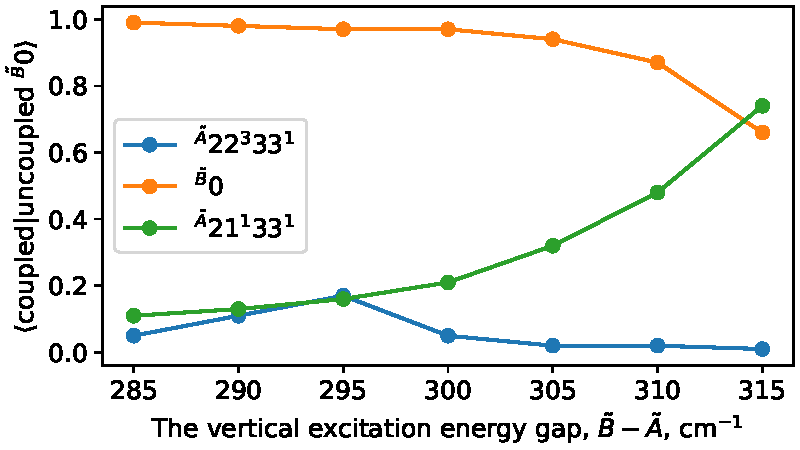
\includegraphics[width=12 cm]{./figures/decomposition.pdf}
    \end{center}
    \caption{
        Dependents of the content of the uncoupled $^{\tilde{B}}0$ state on the
        vertical excitation energy gap between the $\tilde{A}$ and $\tilde{B}$
        states for three states in the proximity of the $\tilde{B}$ state's
        origin.
    }
    \label{fig:decomposition}
\end{figure}

The discussion of the second-order vibronic effects highlights that the
intensity of the vibronic features is strongly tied not only to the strength of
the diabatic couplings but also to the gaps in the vertical excitation energy
between the coupled states. As described in Sec.~\ref{sec:results:parameters}
the \emph{ab inito} error estimate for the gap between the $\tilde{A}$ and
$\tilde{B}$ states has to be at least a few tens of wavenumbers; and indeed the
comparison against the experimental spectrum shows discrepancy of that order.
To estimate the relevance of the vibronic structure findings, this section
presents a study of the sensitivity of the vibronic peaks' character to the
value of the gap between the $\tilde{A}$ and $\tilde{B}$ states.

We focus on the $^{\tilde{B}}0$ state and the two nearest vibronic peaks
resulting from the second-order coupling to the $\tilde{A}$ state: the
$^{\tilde{A}}22^3 33^1$ and $^{\tilde{A}}21^1 33 ^1$ states. These vibronic
states are chosen as they draw the intensity from the $^{\tilde{B}}0$ and are
energetically the closest, therefore these states are expected to show the
strongest response to any changes in vertical excitation energy of the
$\tilde{B}$ state.

Figure~\ref{fig:decomposition} presents changes to the character of the
vibronic peaks as a function of the vertical gap between the $\tilde{A}$ and
$\tilde{B}$ states. The gap is changed by increasing the vertical excitation
energy of the $\tilde{B}$ state while keeping the $\tilde{A}$ state's position
unchanged. The character of the vibronic state is measured as an overlap
between the coupled state and the uncoupled, i.e., Franck-Condon, version of
the $^{\tilde{B}}0$ state, the details of this procedure are described in
Ref.~\cite{Wojcik:ozone:2024}.

The coupled $^{\tilde{B}}0$ state shows significant resemblance to its
uncoupled version. The overlap value drops when the energetic spacing to
another coupled state becomes significant. The curve for the $^{\tilde{A}}22^3
33^1$ state shows that the coupling to the $^{\tilde{B}}0$ state results in a
maximum mixing at the $\tilde{A}$-$\tilde{B}$ gap close to 295~cm$^{-1}$. A
denser sampling in that region would likely reveal an even stronger mixing
between the two states. The case of $^{\tilde{A}}21 ^1 33 ^1$ state is an
example of such stronger mixing, at the values close to 315~cm$^{-1}$ both
states carry equal content of the $^{\tilde{B}}0$ state. The two top,
right-most points on the figure should in fact already switch the colors as the
character of the two states has already changed.

The example of coupling of $^{\tilde{B}}0$ to either $^{\tilde{A}}22^3 33^1$ or
$^{\tilde{A}}21 ^1 33 ^1$ shows how the vibronic effects can lead to a very
bright state leaking as much as half of its intensity to an otherwise dark
state. The difference in the response of $^{\tilde{A}}22 ^3 33 ^1$ and
$^{\tilde{A}21^1 33^1}$ to the position of the $^{\tilde{B}}0$ state shows that
for some dark states the vibronic coupling can produce significant intensity
borrowing even if the positions of the uncoupled states are relatively far
apart (the $^{\tilde{A}}21 ^1 33 ^1$ case), while for other states (the
$^{\tilde{A}} 22 ^3 33^1$ case) the accidental degeneracy of the uncoupled
states is needed in order to observe strong mixing.


\subsubsection{Isotope substitution}
\label{sec:results:simulations:isotope}

\begin{figure}
    \begin{center}
        \includegraphics[width=12 cm]{./figures/SrOPh-duszyński.pdf}
    \end{center}
    \caption{
        Matrix of inner products between the normal modes of the ground state
        of SrOPh and its deuterated version SrOPh-d$_5$. Column and row labels
        show mode frequencies in~cm$^{-1}$.
    }
    \label{fig:sroph_duszynski}
\end{figure}

The Sec.~\ref{sec:results:simulations:gap} discussed the importance of the
value of the vertical energy gap between electronic states in the simulations
of the vibronic effects. The gap changes of the order of tens of wavenumbers
can result in profoundly different intensities of the peak spectra. Similar
observation should apply to the response of the simulated spectrum to the
changes in the frequencies of the uncoupled modes. Instead of considering a
model in which these frequencies are shifted arbitrarily, this section
considers the case of deuterated molecules.

Deuterated strontium phenoxide SrOPh-d$_5$ would be characterized by the same
parameters as SrOPh, except for changes in the normal modes, effectively
allowing to study, also experimentally, the response of the vibronic spectrum
to the shifts in the positions of uncoupled vibrational states.

The changes of the normal modes of the strontium phenoxide due to deuteration
are visualized on figure~\ref{fig:sroph_duszynski}. The figure presents the
matrix of inner products between the two sets of normal modes, also known as
the Duschinsky rotation matrix. The columns and rows of the matrix additionally
list the harmonic wavenumbers of the corresponding modes. The figure shows
that the lowest frequency modes remain largely unchanged in the deuterated
molecule and can still be identified as various displacements of the Sr-O-C
group of atoms. The harmonic wavenumbers of the deuterated modes lower by
about 5\%. The medium-frequency modes change not only its frequencies but also
its shape, however, none of these modes was significant for the simulations
discussed earlier.

The main focus of this section is to view the changes in the vibronic spectra
due to small changes in the positions of uncoupled states. As described in the
previous paragraph deuteration of the molecule allows to achieve the exact
effect.

\begin{figure}
    \begin{center}
        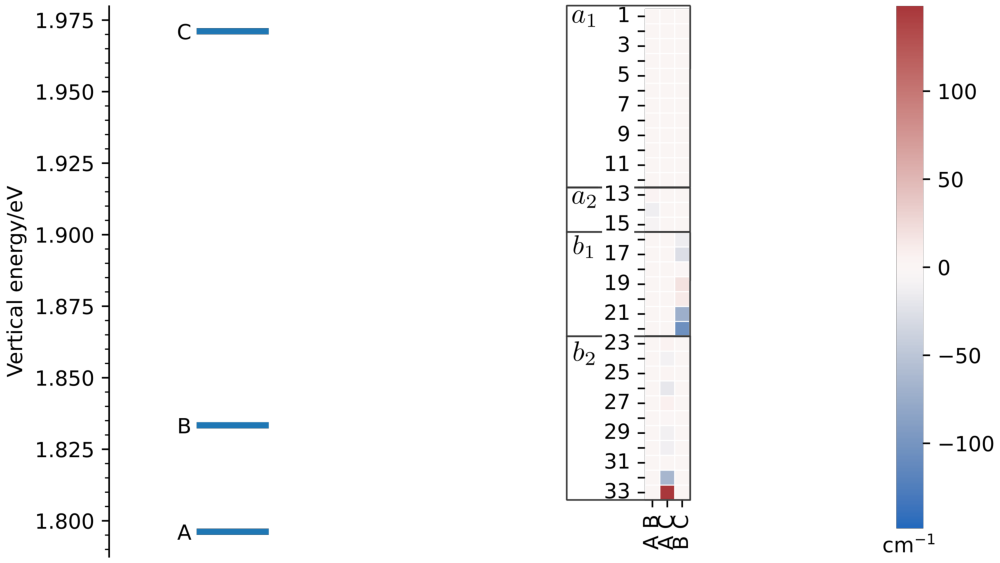
\includegraphics[width=12 cm]{./figures/SrOPh5dCouplings.pdf}
    \end{center}
    \caption{
        Diabatic couplings for SrOPh-d$_5$, compare to
        figure~\ref{fig:SrCouplings}.
    }
    \label{fig:srd5_couplings}
\end{figure}

With the changes of the normal modes, the expansion coefficients of the KDC
Hamiltonian, Eqs.~\eqref{eq:kdc_Voff} and \eqref{eq:kdc_Vdiag} change as well.
Figure~\ref{fig:srd5_couplings}, presents the changed values and structure of
the diabatic couplings. The key qualitative properties are preserved, i.e.,
strong coupling of $\tilde{A}$-$\tilde{C}$ states along $\nu _{33}$, strong
coupling of $\tilde{B}$-$\tilde{C}$ states along $\nu _{22}$ and $\nu _{21}$,
and vanishing couplings between $\tilde{A}$-$\tilde{B}$. Quantitatively, the
couplings strengths become a little weaker. Overall, the consequence of this
change is that the comparison between the deuterated and undeuterated molecules
probes a few more parameters of the KDC Hamiltonian than only the position of
uncoupled vibronic states.

\begin{figure}
    \begin{center}
        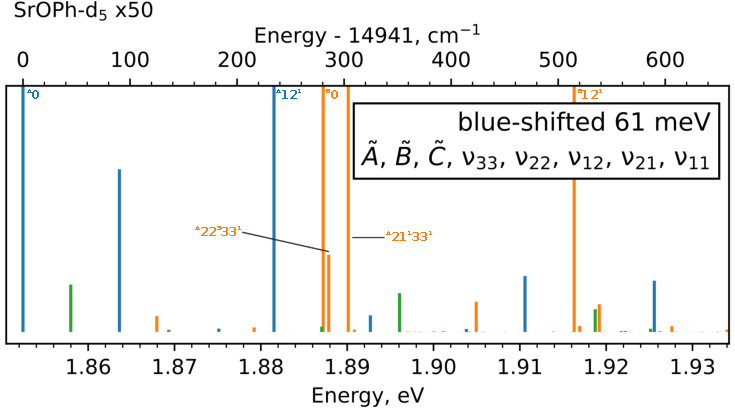
\includegraphics
        [width=12 cm]
        {./figures/SrOPhd5_0t650_zoom_annot_Mulliken.pdf}
    \end{center}
    \caption{
        Vibronic absorption spectrum of SrOPh-d$_5$, compare with the
        undeuterated spectrum from figure~\ref{fig:SrOPh_0t650_assigned}.
        Annotations mark the peaks discussed in
        Sec.~\ref{sec:results:simulations:gap}.
    }
    \label{fig:Srd5_spectrum}
\end{figure}

The simulated spectrum of the deuterated molecule is presented on
figure~\ref{fig:Srd5_spectrum}. The progressions discussed in
Sec.~\ref{sec:results:simulations:linear} remain largely unchanged upon the
deuteration with the only difference appearing due to the small frequency
shifts of the deuterated modes. There are however two states that respond to
the deuteration far stronger, these are the same sates as discussed in
Sec.~\ref{sec:results:simulations:gap}, the $^{\tilde{A}}22^3 33^1$ and
$^{\tilde{A}}21^1 33^1$. For both of them the small change in the frequency is
met with a significant increase in their intensity, as the shift moves both
sates closer to the bright $^{\tilde{B}}0$ peak.

\section{Summary}

The vibronic effects present in strontium phenoxide make many
Franck-Condon-forbidden transitions allowed. Modeling of the vibronic effects
in the absorption spectrum of SrOPh using the KDC Hamiltonian in a diabatic
basis of Ichino, Gauss, and Stanton reveals that the second order effects lead
to significant mixing of the origin band of the $\tilde{B}$ state with the
neighbouring states hosted on the $\tilde{A}$ state. These couplings are very
sensitive to the exact values of the model parameters such as the vertical
excitation energies or harmonic frequencies of the normal modes. The modulation
of harmonic frequencies that is afforded by the deuteration of the phenoxide
group helps to connect the experimentally observed vibronic features with the
modeled couplings scheme.

The \emph{ab initio} calculations show that the vertical excitation
energy of the $\tilde{C}$ state is more sensitive to the basis set size and
level of correlation than the $\tilde{A}$ and $\tilde{B}$ states.

\newpage
\printbibliography{}

\end{document}

% vim: wrap lbr spell:
